\section{Introduction}

\todo{} 

We are using the task of hitting targets precisely with a whip as a case study for dynamic manipulation of deformable object. This is a challenging task due to following factors: 
\begin{itemize}[leftmargin=3mm]

\item \textbf{Complex object properties:} Unlike \ben{a} rigid object, the motion of a deformable object is influenced by many more factors such as stiffness, aerodynamic, density distribution, where many of these parameters are notoriously difficult to model or measure. \shuran{missing the aspect of high dof, under-actuated}
Therefore, prior studies are often confined to known objects and fail to generalize to new objects with different properties. 

\item \textbf{Complex dynamics:} Unlike quasi-static manipulation, dynamic manipulation is ??  (action - trajectory, instead of action - position? ) %less predictable -- same action same rope can result in different trajectory due to different initial conditions. This uncertainty varies with respect to action, goal configuration and rope parameters, requiring the system to explicitly model this uncertainty and plan its action accordingly. 
\shuran{maybe this complex action object property relationship can be mentioned here?}
\ben{Ben: I think this misses some of the aspects that make deformable objects (and cloth in particular) so interesting and challenging. While cloths and whips have virtually infinite degrees of freedom in principle, at any given time the \textit{effective degrees of freedom} are highly dependant on the action being taken and contact between the object and environment. A whip moving at high speed in a circular motion is, for all intents and purposes, temporarily fully actuated and has essentially only 6 degrees of freedom (i.e. it's rigid). In contrast to rigid objects, dynamics affects not only the object's interaction with its environment but also the effective kinematics of the object itself.}


\item \textbf{Precise goal condition:}  Due to these challenges, prior works on dynamic deformable object manipulation focus tasks that has a lower precision requirement (e.g., cloth unfolding \cite{ha2021flingbot}, or cable vaulting \cite{zhang2021robots}). In contrast, our task require the system to produce accurate actions in order to precisely reaching goal condition (i.e., hitting the goal position with \the tip of a whip). \ben{Ben: I think this bullet conflates two things. 1: The how many distinct behaviors can achieve a goal and 2: How precise is the goal. It's possible that a very precise goal can still be achieved with multiple very different policies/strategies/trajectories.}

\end{itemize}


\begin{figure}[t]
    \centering
    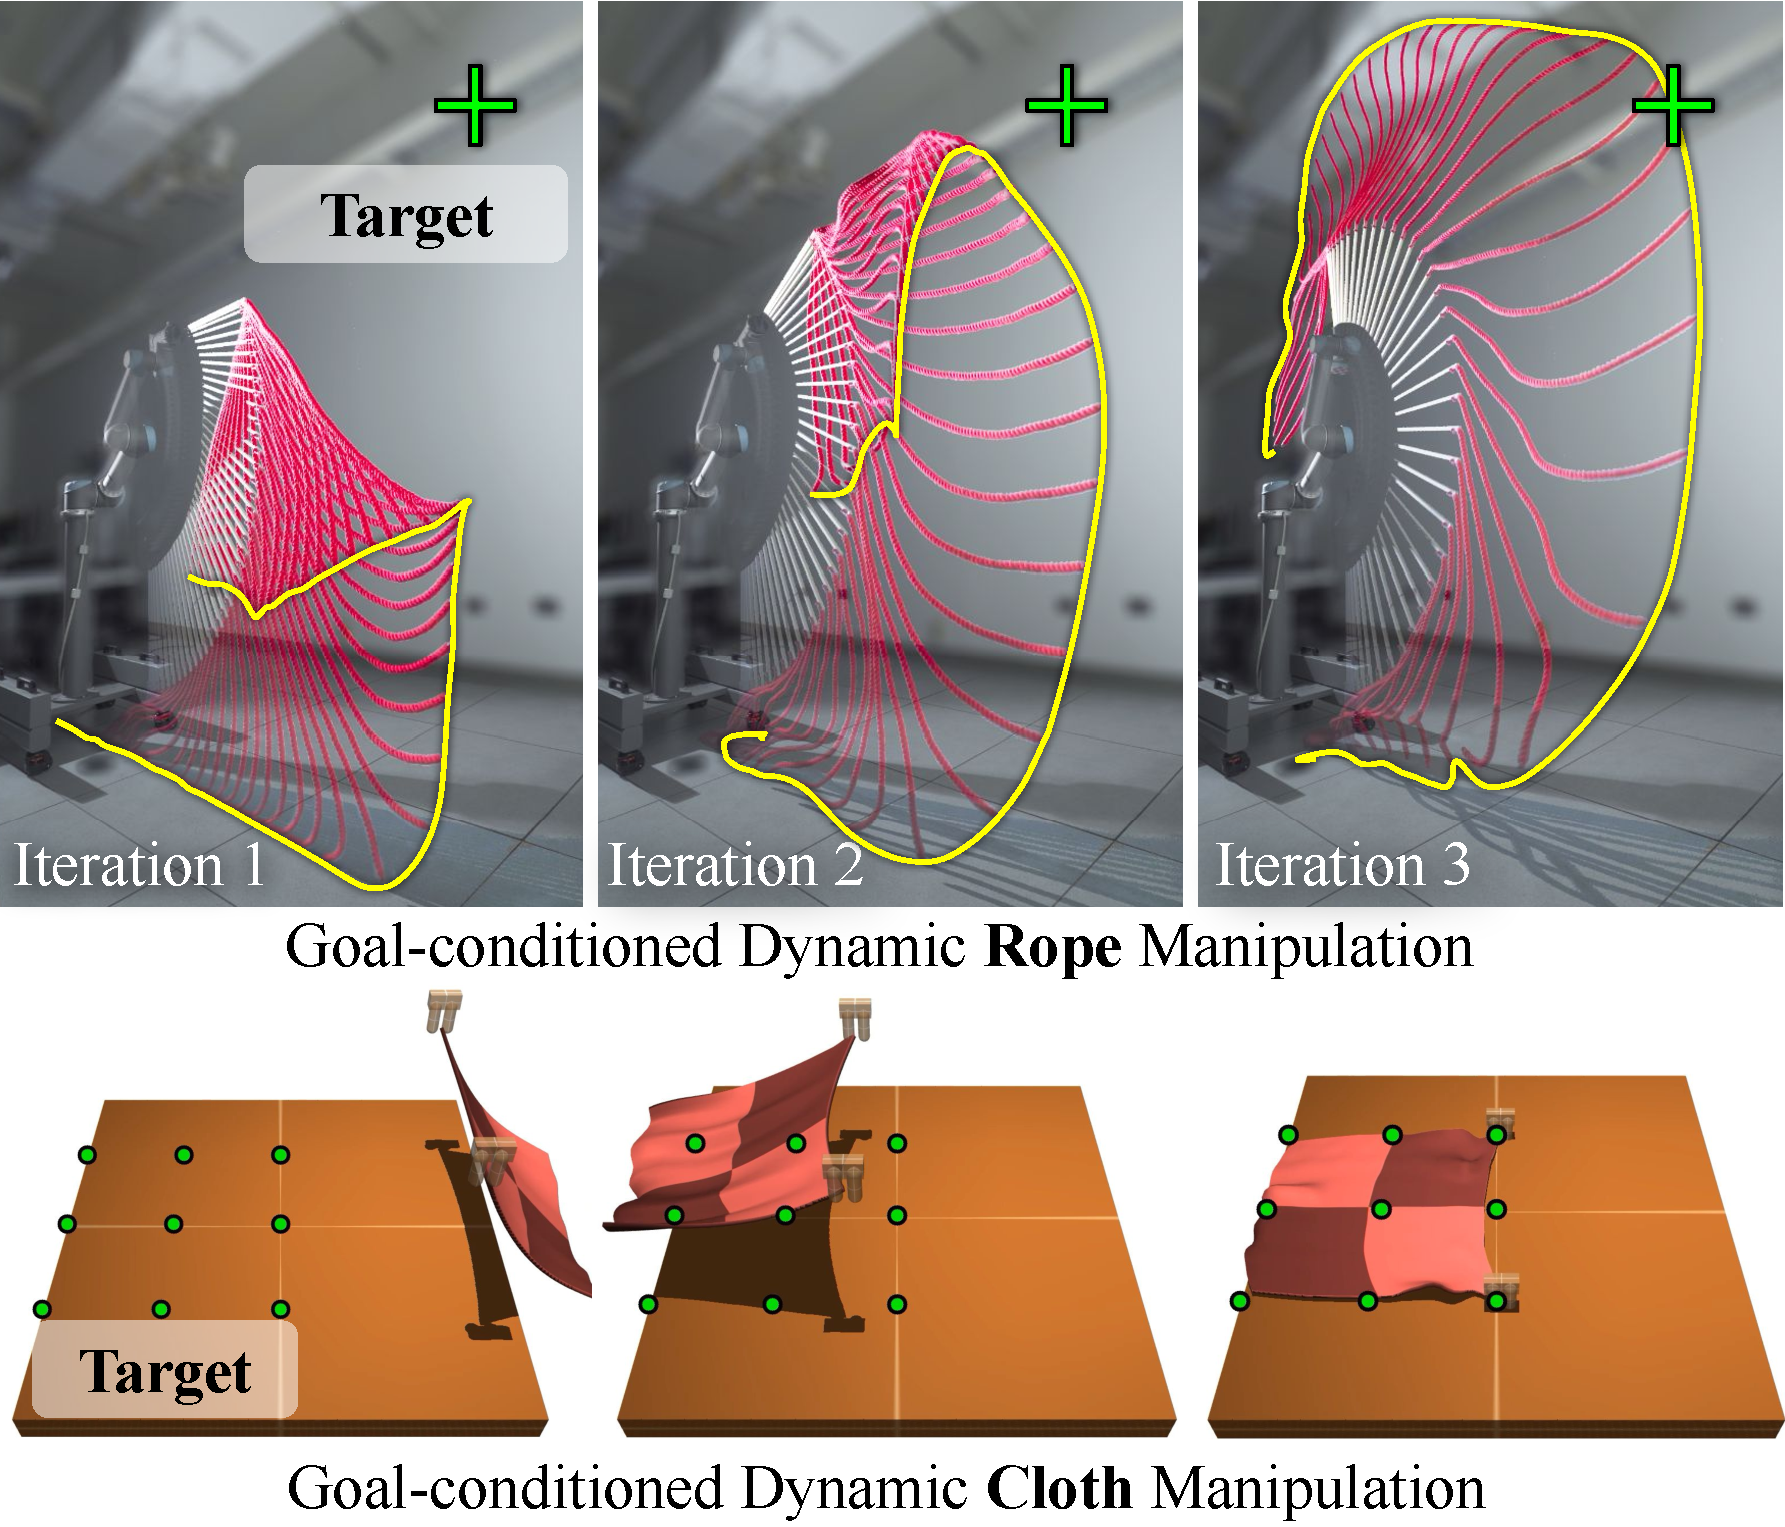
\includegraphics[width=\linewidth]{figure/rope-teaser.pdf}
    %https://docs.google.com/drawings/d/12tlTQ5S-eEHEXbHswpW1-dkgyWmvPPUlsDF5sNXWmwo/edit?usp=sharing

    \caption{(Place holder) Teaser Tasks, Realworld Robot + Rope figure.  highlight the iterative process, trajectory for step 1,2,3,4.  \todo{caption}
    }
    \label{fig:task}
\end{figure}


In this work, we present \textbf{\namel~(\names)}, an self-supervised formulation that learns how to plan control parameters for whipping a deformable rope  from visual observations. 
\todo{summary of how the system works}
This formulation highlight two key features: 
\begin{itemize}[leftmargin=3mm]
\item \textbf{Residual trajectory representation}: Instead of trying to capture the entire dynamical system and identify key physical parameters, \names~only learns how a given trajectory will deform under small changes in action. This formulation efficiently reuses the rich physical information captured by the observation, which allows the model to generalize to unseen ropes with significantly different dynamics comparing to training data.
\shuran{"reuses the rich physical information captured by the observation", why?}

\item \textbf{Iterative Action Improvement}: Instead of learning the direction mapping from the goal to the final action, \names~starts with an rope-agnostic action initialization and selects the best delta action sample that would lead towards the goal. The system then continues to readjust its actions base on the new observations. For tasks with repeatable actions, this iterative approach allows the system to achieve high precision and robust against errors from action, observation and model prediction.


% \item \textbf{Implicit system representation}: %what we do, what's the advantage. 
% Instead of explicitly model the object physical properties, \names~learns a implicit latent representation of the deformable object from a sequence of visual observation under dynamic interaction. This formulation allows the model to learn most relevant object feature representation through active interaction, which is more flexible than a set of predefined physical parameters and easier to adapt to new scenarios.  

% \item \textbf{Residual action inference:} %what we do, what's the advantage.
% Instead of learning the direct mapping from the goal to the final action, \names~starts with an random action initialization and infers delta action at each step that would lead towards the goal. The system then continues to readjust its actions base on the new observations. This iterative approach is what allows the system to achieve precise prediction and control for this highly dynamical and complex task, since predicting trajectory deviation for small delta action is much easier than memorizing trajectory for all possible actions.
\end{itemize}

This formulation provide a  general framework for precise dynamic manipulation that allows  efficient generalization for varying rope properties, robot hardware parameters.  Thanks to its adaptable formulation, the model trained in simulation can be directly applied to realworld robot platform with online adaptation.  

In summary, our  primary contribution is the \namel~(\names), an self-supervised formulation that learns how to plan control parameters  for dynamically manipulating (whipping) a deformable rope  from visual observations. 
We demonstrate this framework in the task of xxx. 
Our experiment shows ... 


\iffalse
\textbf{Problem:}
\begin{itemize}    
    \item{Difficult to model dynamics}: High degrees of freedom with non-linear dynamics and difficult to measure parameters. \textbf{Hard to compute Jacobian analytically.} This makes model-based control/RL difficult. \textbf{Large sim-to-real gap.}
    
    \item{Difficult to plan/control}: Highly underacutated. Goal can not be mapped trivially to actions.
\end{itemize}

\textbf{Solution:}
\begin{itemize}
    \item{Learning the notion of Jacobian} for \textbf{online adaptation}. Intuitive physics.
    \item{Identical input and output representation} easier to learn, better generalization.
    \item{Motion primitive} to reduce action space.
\end{itemize}

\textbf{Contribution:}
\begin{itemize}
    \item{First to solve a task} Goal conditioned dynamic manipulation of deformable.
    \item{A method to close the sim-to-real gap} Representation to enable online adaptaion.
\end{itemize}

\textbf{Key takeaway:}
\begin{itemize}
    \item{Learned close-loop policy transfer better}
    \item{Decouple goal and learning}
    \item{}
\end{itemize}


% Current literature interpreters the term intuitive physics in different ways. 
% 1. Object permance
% 2. Learning output of physics simulation or residual
% 3. Predict next state given current state and action

% Our work is more in-line with clever reformulation of the original problem for easier learning.
% And turn problem into class 3.
\fi 

\begin{figure*}[t]
    \centering
    \includegraphics[width=0.49\linewidth]{example-image-golden}~\includegraphics[width=0.49\linewidth]{example-image-golden}
    \caption{Challenges: (1) Show trajectory of whipping 3 different rope with same action (different stiffness, mass distribution) (2) Same rope same action, executed in 10 times, show the averaged trajectory for uncertainty (? if we don't handle uncertainty, don't include this). }
    \label{fig:task}
\end{figure*}